\section{Methods}
\subsection{Participants}
119 participants were recruited from the university campus, with 69.74\% identifying as 'male', 28.57\% as 'female' and 1.68\% as 'other'.
Participants were aged between 18 and 27, the average age was 22 years, with a standard deviation of 2.4 years.
The study programs most frequently represented were computer science, software engineering and aerospace engineering.
Participants each received €15 as monetary compensation for their involvement in the study.

\subsection{Design}
This study employed a $2 \times 8$ factorial design, examining the impacts of gamified elements and participant gender on performance and anxiety within a digital learning environment.
The independent variables were gamified elements and gender.
For gamified elements, participants were assigned to one of the following eight conditions: No Gamification (None), Points (P), Badges (B), Leaderboards (L), Avatars (A), Narrated Content (N), Points-Badges-Leaderboards-Avatars (PBLA) and Points-Badges-Leaderboards-Avatars-Narrated Content (PBLAN).
The gender variable was measured categorically with participants identifying as male, female, or other.
Each participant experienced three iterations with different conditions, chosen randomly from a pre-generated set to ensure a balanced distribution across conditions and gender, reflecting a within-subjects design element.
This setup allowed for the analysis of interaction effects between gamified elements and gender on the dependent variables, which were performance and anxiety.
The study aimed to isolate the effects of gamification components in learning, controlling for gender differences.

\subsection{Materials}
\subsubsection{Physical environment}
The study was conducted in two separate rooms in the cellar of a university building, one equipped with five and one with seven iMacs.
As \textcite{christyLeaderboardsVirtualClassroom2014} suggested that the physical environment can influence the results, both rooms were equipped with the same furniture and lighting and were furnished very dry, like a typical software laboratory.

\subsubsection{Virtual environment}
The software used in this study was built by the author using SvelteKit in frontend and KTor in backend. Its UI was designed after the study by \textcite{albuquerqueDoesGenderStereotype2017}.
On the iMacs the study was displayed full-screen mode using the Safari web browser to ensure no further distractions. The study consisted of 7 screens.
A consent screen gave an overview and explained the data collection to the user. The consent screen had to be accepted in order to proceed.
A demographic data screen collected gender, age and study program. Participants also had to enter a deletion code in order to request their data's deletion after the collection.
\begin{figure}[H]
  \centering
  \includegraphics[width=0.5\textwidth]{img/details.png}
  \caption{The personal details collection form}
  \label{fig:figureDetails}
\end{figure}
The next screen was the gamified learning environment, where the participants had to solve 20 questions in a row while being exposed to the gamified elements.
The matrices were taken from \textcite{albuquerqueDoesGenderStereotype2017}, to generate 60 questions out of the 20, the 40 questions for iteration two and three were slightly altered versions of the original 20 made by this author.
Those alterations included changing the position or rotation of the elements in the matrix and the five possible answers.
\begin{figure}[H]
  \centering
  \begin{subfigure}[t]{0.4\textwidth}
    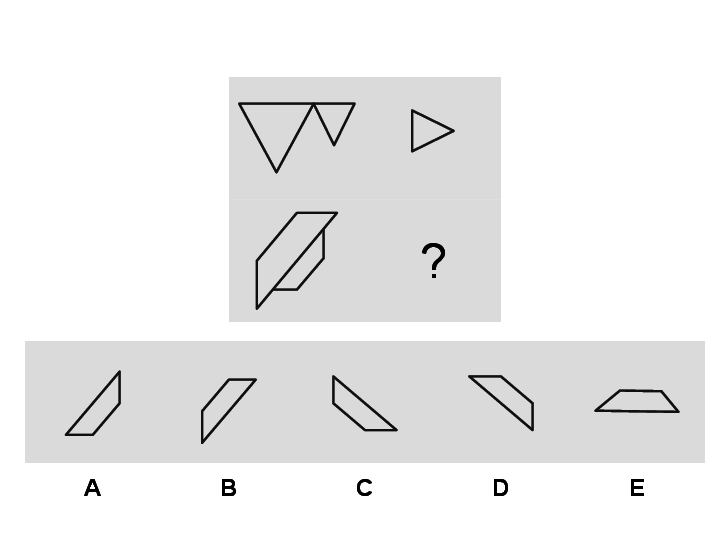
\includegraphics[width=\textwidth]{img/q-17.png}
    \label{fig:figureMatrixStandard}
  \end{subfigure}
  \hspace{5mm}
  \begin{subfigure}[t]{0.4\textwidth}
    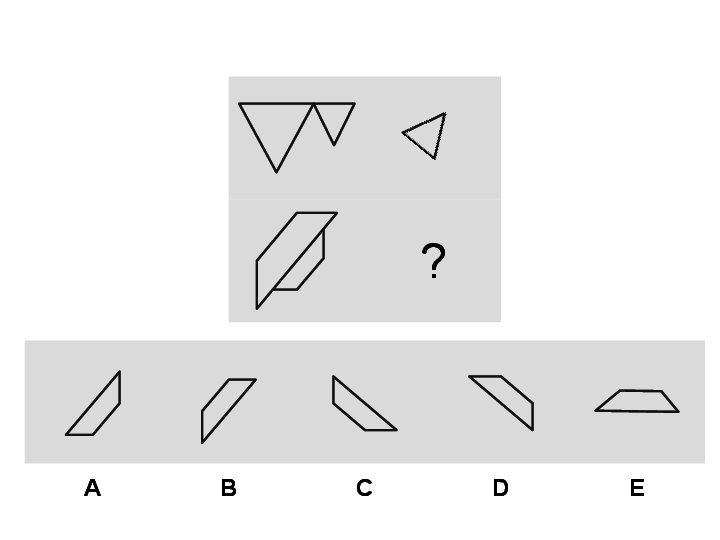
\includegraphics[width=\textwidth]{img/q-57.png}
    \label{fig:figureMatrixAltered}
  \end{subfigure}
  \caption{Left: A standard progressive matrix from \textcite{albuquerqueDoesGenderStereotype2017} given to the participants. Right: A slightly altered version of the same matrix}
  \label{fig:figureMatrices}
\end{figure}
The gamified learning environment consisted of different UI elements representing the gamified elements.
\begin{APAitemize}
  \item \textbf{Leaderboards}: A list of participants and scores, including the current participant. The other players shown were not real.
  \item \textbf{Badges}: An array of four badges that were awarded for 1, 5, 10 and 18 correctly answered questions.
  \item \textbf{Avatars}: A small avatar that was shown in the top right corner of the screen and on the leaderboard. To increase identification with the avatar further, the participants were asked to choose one of 15 different avatars before the iteration.
  \item \textbf{Narrated content}: Narrated content was shown in the bottom right corner of the screen. It was presented as a speech bubble with an avatar next to it, in case avatars were enabled. It showed a random praise or encouragement sentence every three questions.
  \item \textbf{Points}: A counter next to the question frame showed the current points. One point was awarded for each correctly answered question.
\end{APAitemize}
\begin{figure}[H]
  \centering
  \begin{subfigure}[t]{0.4\textwidth}
    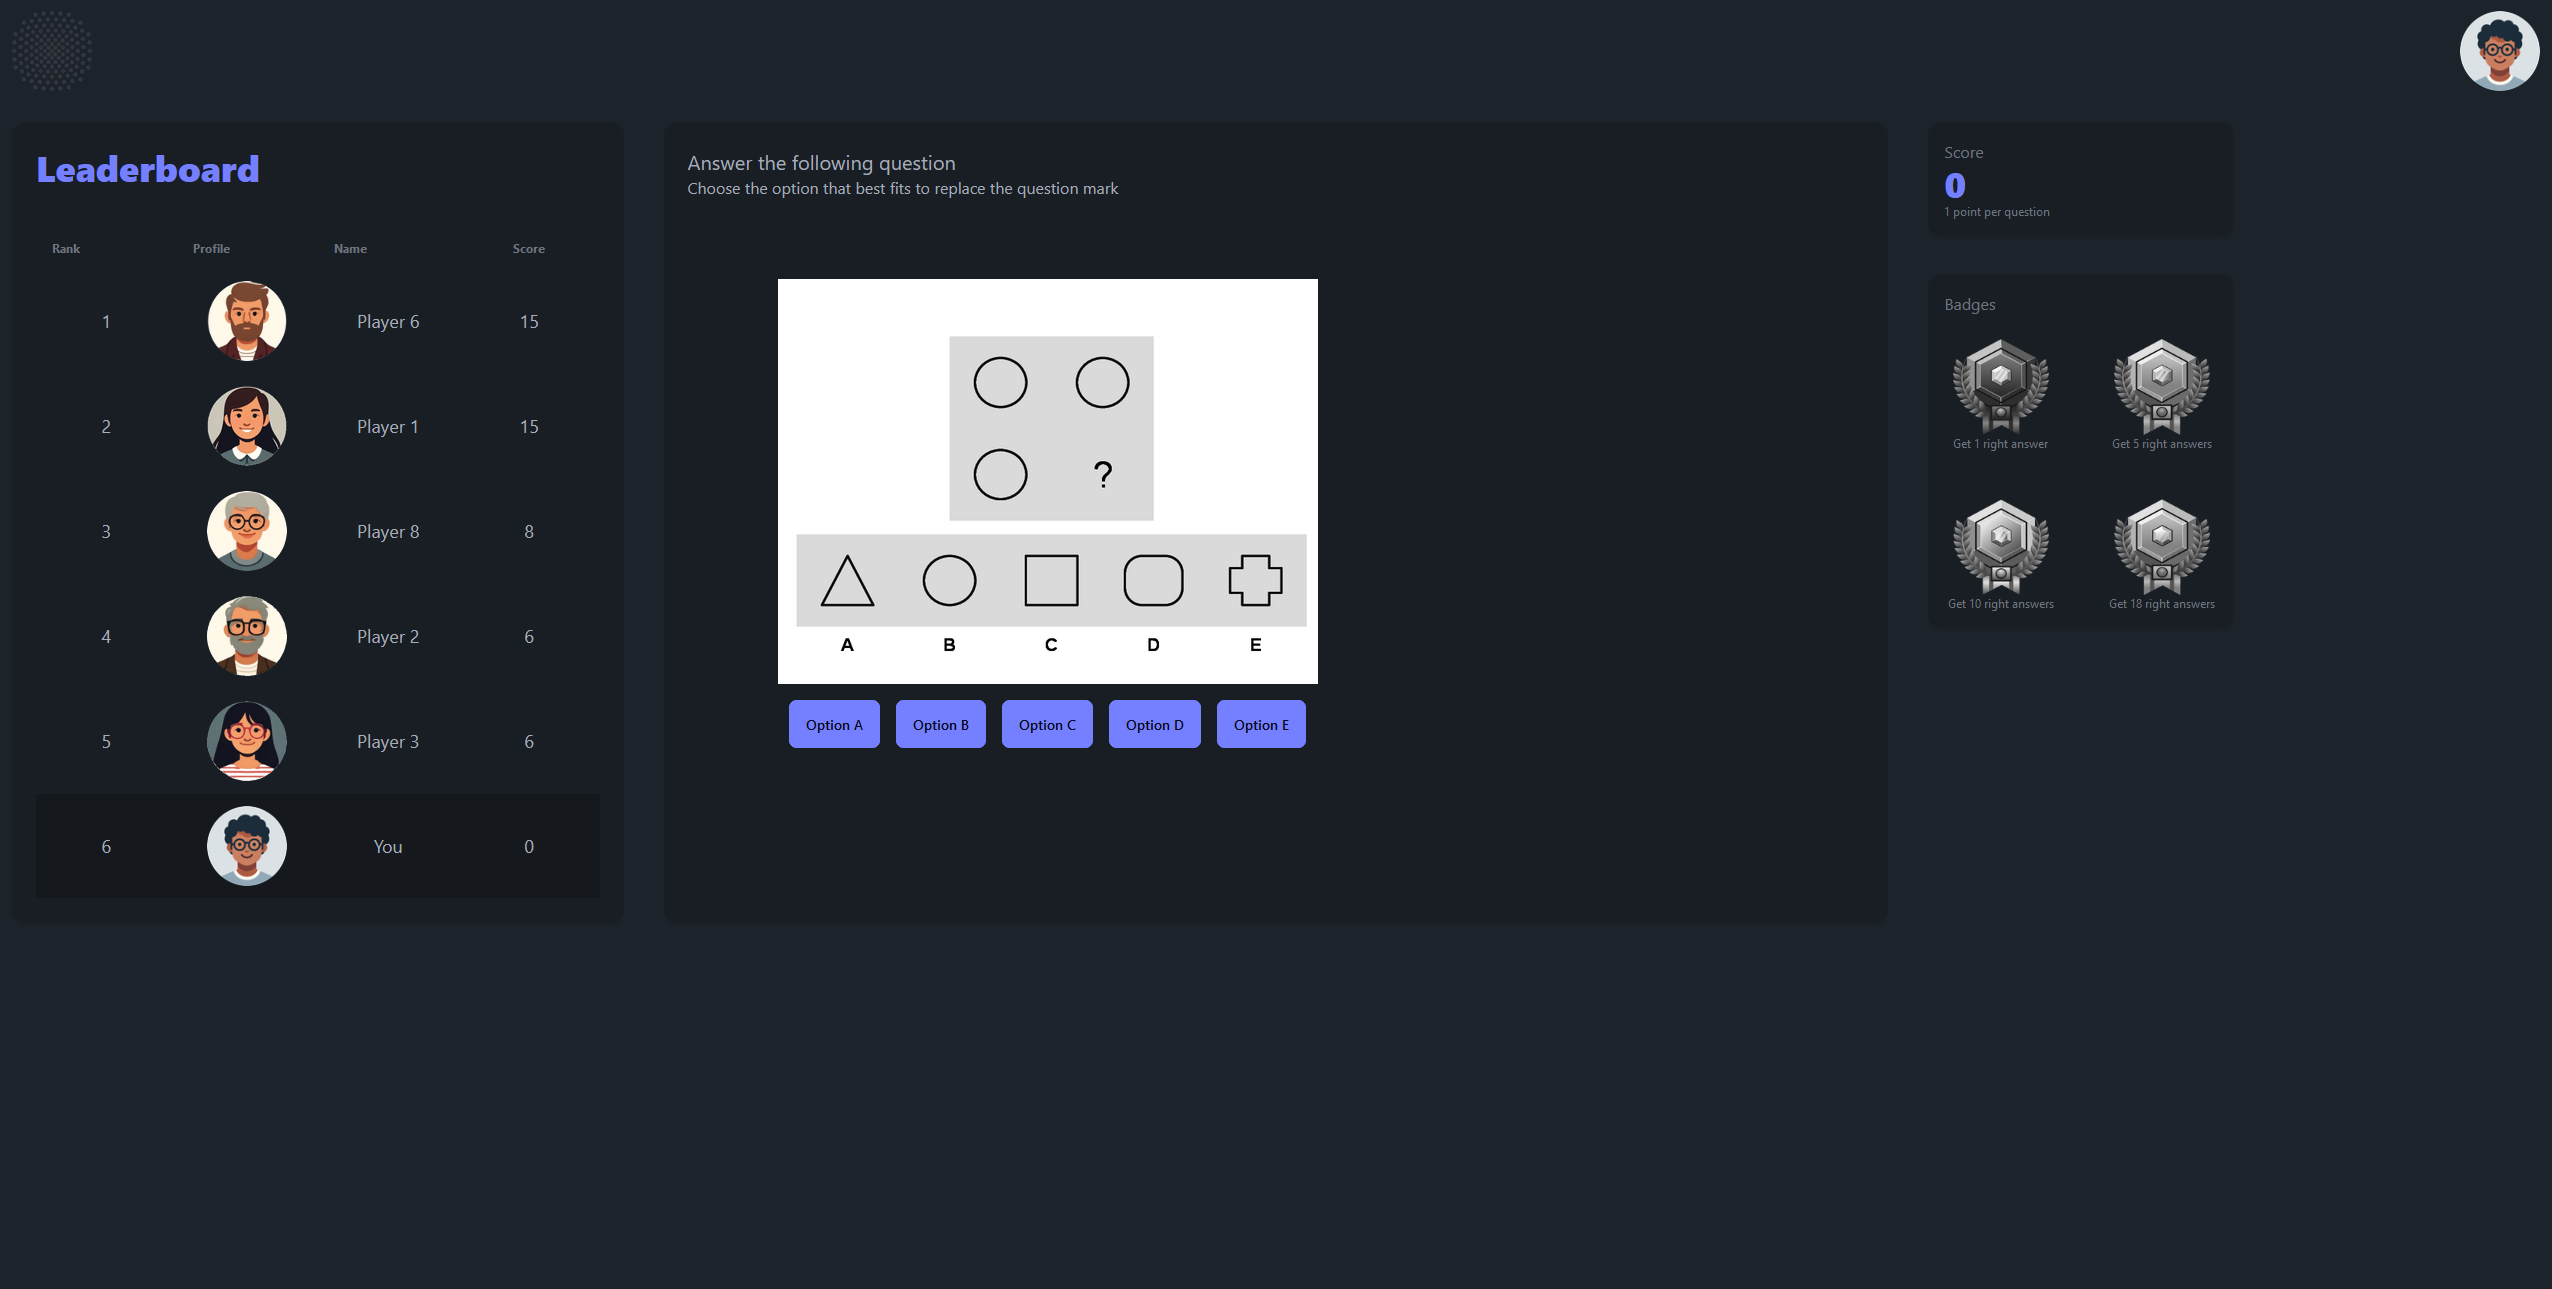
\includegraphics[width=\textwidth]{img/question_screen.png}
    \label{fig:figureScreenEnabled}
  \end{subfigure}
  \hspace{5mm}
  \begin{subfigure}[t]{0.4\textwidth}
    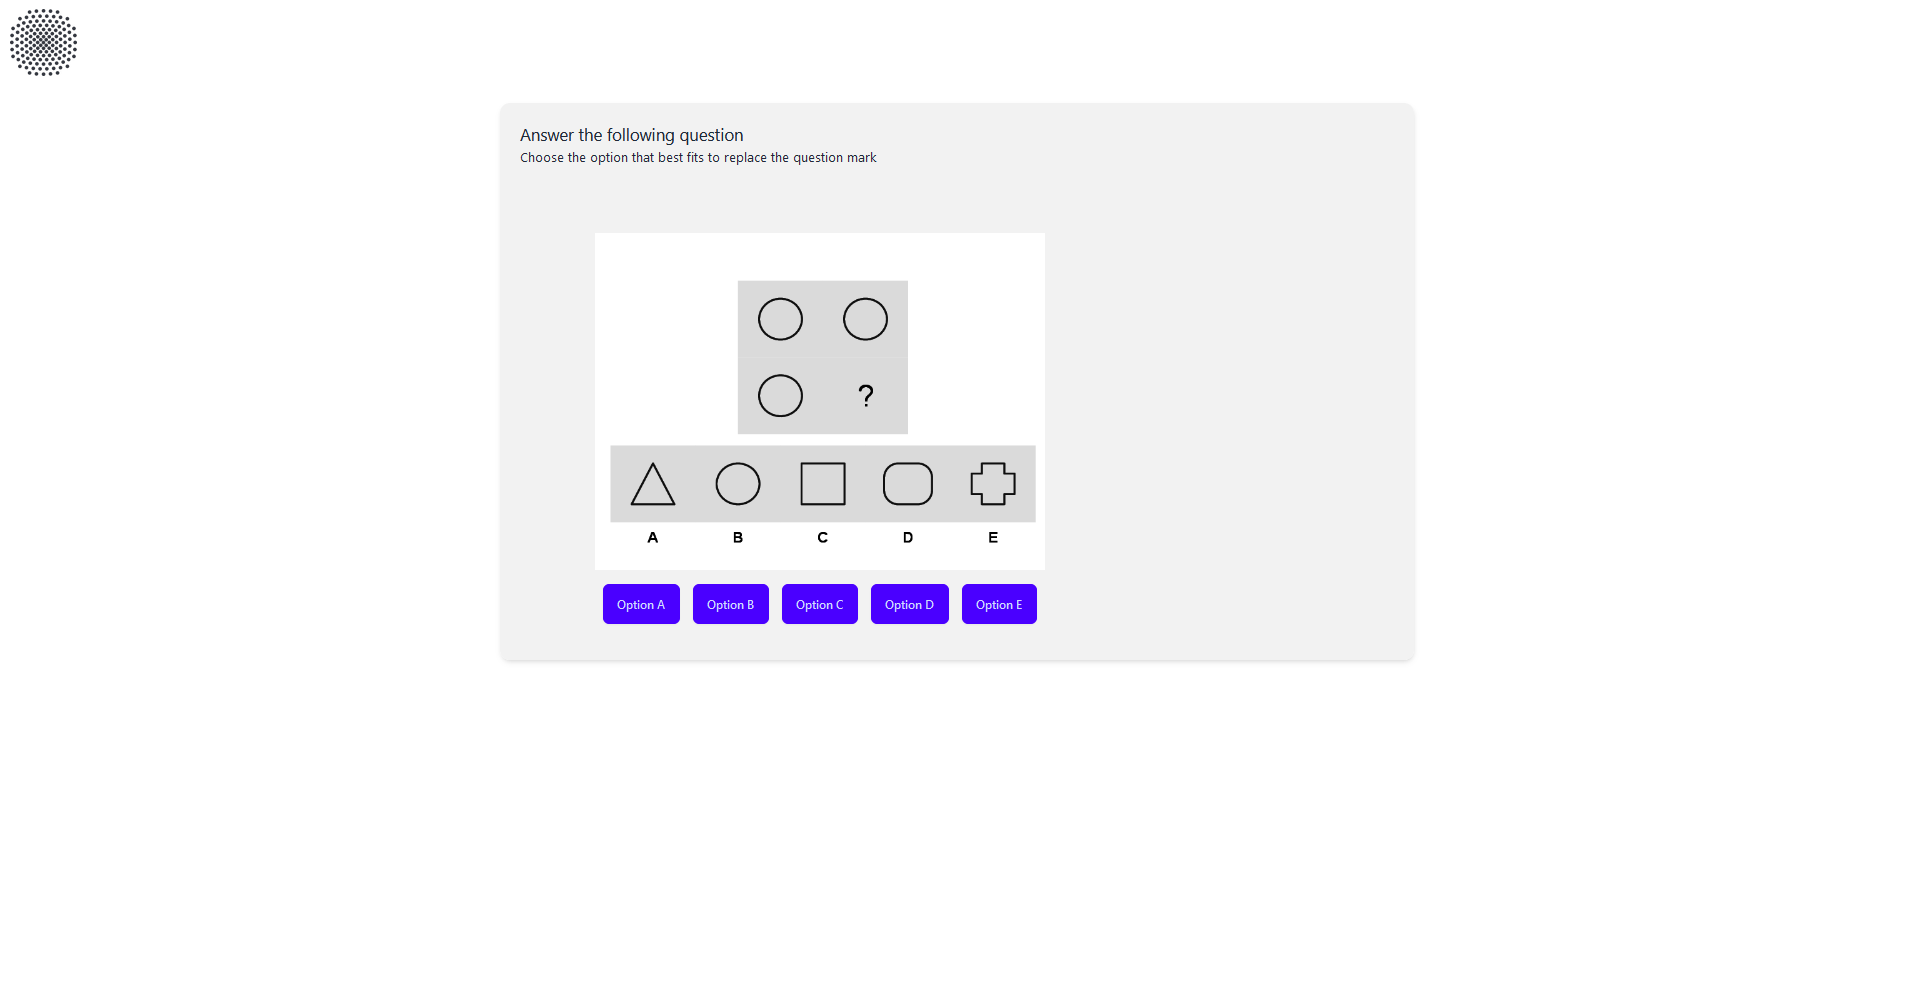
\includegraphics[width=\textwidth]{img/question_screen_no_elements.png}
    \caption{The Digital Learning Environment with no Gamified Elements enabled}
    \label{fig:figureScreenDisabled}
  \end{subfigure}
  \caption{Comparison of the Digital Learning Environment with gamified elements enabled (left) and without gamified elements enabled (right). Narrated content in only shown between questions so it is not possible to show it in the same screenshot.}
\end{figure}

After the gamified learning environment, the participants were shown a questionnaire for anxiety, motivation and self-efficacy.
The three questionnaires were a six-question shortened form of the State-Trait Anxiety Inventory (STAI) \parencite{marteauDevelopmentSixitemShortform1992}, the eight-question General Self-Efficacy Scale (GSE) \parencite{guayAssessmentSituationalIntrinsic2000} and the 16-question Situational Intrinsic Motivation Scale (SIMS) \parencite{chenValidationNewGeneral2001}.
\begin{figure}[H]
  \centering
  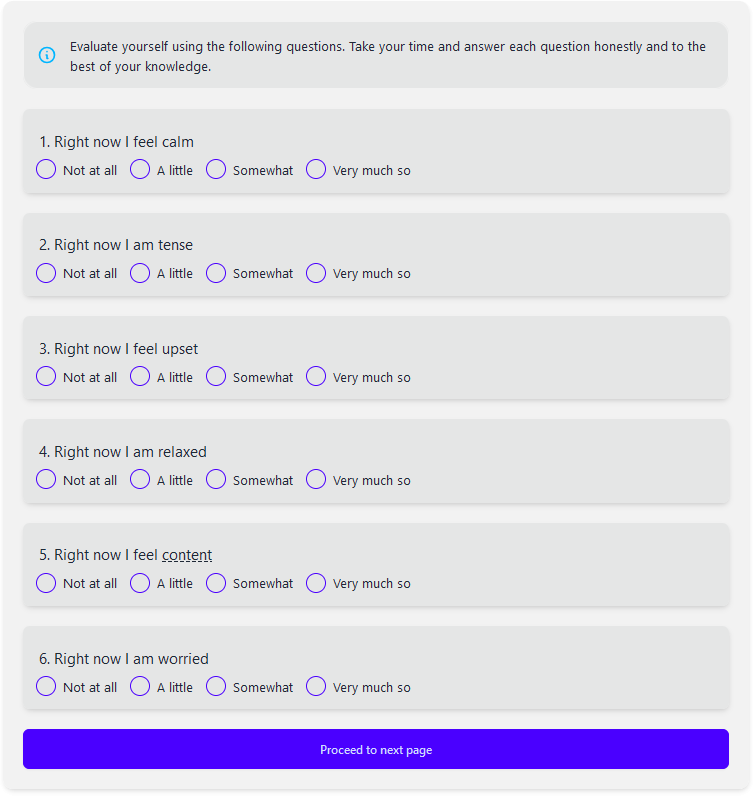
\includegraphics[width=0.4\textwidth]{img/Stai.png}
  \caption{The anxiety questionnaire}
  \label{fig:figureAnxiety}
\end{figure}
To submit data to the backend there was a data submission screen that guided the participants to the next iteration or in case of the third iteration to the end of the study.

\subsection{Procedure}
\begin{figure}[H]
  \centering
  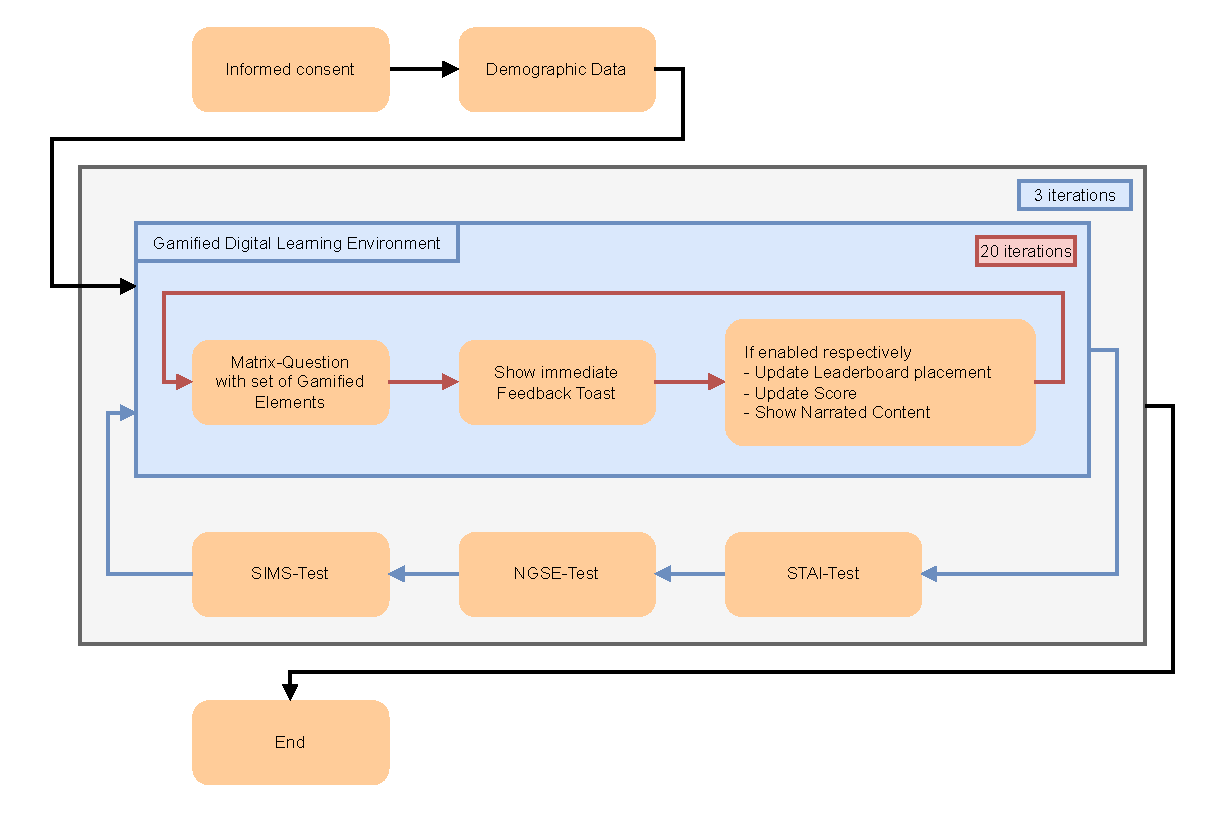
\includegraphics[width=\textwidth]{img/Procedure_alt.pdf}
  \label{fig:figureDetails}
\end{figure}
Participants have been enlisted at the university campus and invited to engage in a study concerning gamification, with an incentive of 15€ offered upfront for their involvement.
Following a brief overview of the study's framework, they have been directed to select both a room and a computer.
The initial screens presented were those seeking consent and outlining the study details and the demographic data collection screen. Subsequently, participants have inputted their demographic data, leading into the three gamified iterations.
Each iteration has initiated with the gamified learning environment, followed by three questionnaires, and concluded with a data submission interface.
After answering one question the next question has a one-second delay which increases to four seconds if narrated content is shown.
The sequence and consistency of the testing procedure, including the series of questions asked in the gamified digital learning environment have always been maintained to ensure the reliability of measurements and comparability of results across the various stages of the experiment.
Participants have been advised to proceed at their own pace and refrain from communicating with fellow participants throughout the duration of the study.
Upon completion of the third iteration, they have been acknowledged for their contribution and compensated with the 15€.

\subsection{Scoring}

The data was cleaned and processed before analysis to ensure accuracy and reliability. The scores for the different conditions were calculated as follows:

\begin{APAitemize}
\item \textbf{Performance:} Performance was calculated as the ratio of correctly answered questions to the total number of questions. If this ratio was below 0.25 for any dataset, that dataset was excluded from further analysis. This threshold ensures that only participants with a sufficient level of engagement are included in the study.
\item \textbf{State-Trait Anxiety Inventory (STAI):} The STAI scores were calculated using the six-item short-form version of the State scale, as developed by \textcite{marteauDevelopmentSixitemShortform1992}. Participants rated their responses on a scale from "Not at all" to "Very much so," corresponding to numerical values from zero to five. The original test contains both anxiety-present and anxiety-absent items, with appropriate weights applied as per the guidelines by \textcite{marteauDevelopmentSixitemShortform1992}. Negative weights were used for items indicating anxiety (e.g., "Right now I am worried").
\end{APAitemize}